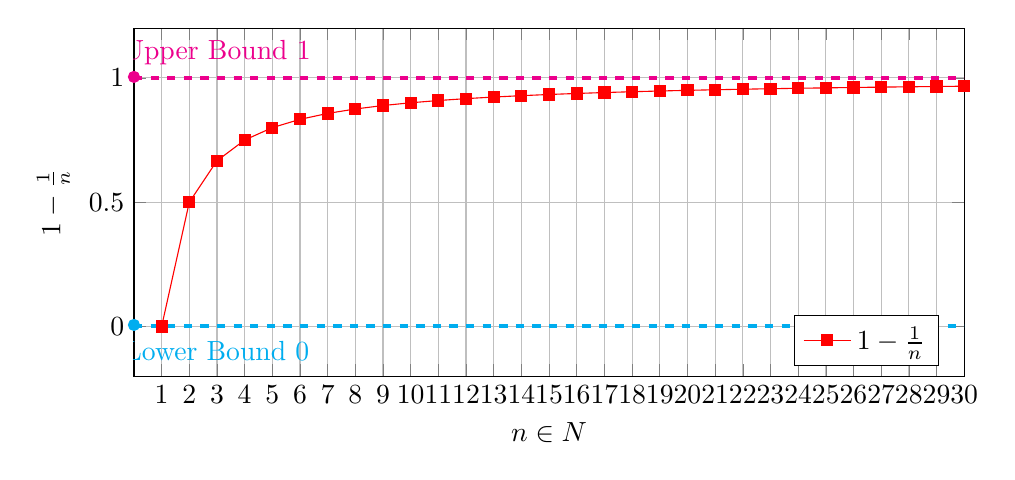
\begin{tikzpicture}
	\begin{axis}[
		xlabel={$n \in \mathbb{N}$},
		ylabel={$1 - \frac{1}{n}$},
		ymin=-.2, ymax=1.2,
		xmin=0, xmax=30,
		xtick={1,2,...,30},
		ytick={0,0.5,1},
		grid=major,
		width=\textwidth,
		height=6cm,
		domain=1:30,
		samples=30,
		legend pos=south east
		]
		% Plot points for 1 - 1/n
%		\addplot[line width=.25mm, only marks, red, mark=x] plot (\x, 1 - 1/\x);
		\addplot[red, mark=cube*, mark options={fill=red}] plot (\x, 1 - 1/\x);
		\addlegendentry{$1 - \frac{1}{n}$};
		
		% Draw horizontal line showing upper bound (y=1)
		\addplot[dashed, magenta, line width=.5mm] coordinates {(0,1) (30,1)};
		\node[magenta] at (axis cs: 3,1.1) {Upper Bound $1$};
		
		% Draw horizontal line showing lower bound (y=0)
		\addplot[dashed, cyan, line width=.5mm] coordinates {(0,0) (30,0)};
		\node[cyan] at (axis cs: 3,-0.1) {Lower Bound $0$};	
	\end{axis}
	\filldraw[magenta] (0,3.8) circle (2pt);
	\filldraw[cyan] (0,.65) circle (2pt);
\end{tikzpicture}